\documentclass{article}
\input{setting.tex}

\title{Reinforcement Learning Assignment 1}
\author{Ali Abbasi -- 98105879}
\begin{document}
\maketitle
\tableofcontents
\pagebreak

\section{}
\subsection{}
Let \(R_{\max}\) be the maximum reward that can be obtained in the environment. Then, we have:
\begin{align*}
V_k^*(s) &= \E{ r_1 + \gamma r_2 + \gamma^2 r_3 + \cdots + \gamma^{k-1} r_k | s_0 = s }\\
&\le \E{R_{\max} + \gamma R_{\max} + \gamma^2 R_{\max} + \cdots + \gamma^{k-1} R_{\max} | s_0 = s}\\
&= \frac{R_{\max} \left(1 - \gamma^k\right)}{1 - \gamma}\\
&\le \frac{R_{\max}}{1 - \gamma}
\end{align*}

\subsection{}
Since the rewards are non-negative, we can act like the policy achieved by \(V_k^*\), and for the \(k+1\)th step, we can choose a random action! If we name this policy \(\pi\), we have:
\begin{align*}
V_{k+1}^{\pi}(s) = V_{k}^*(s) + \underbrace{\gamma^k \E{r_{k+1}|s_0 = s}}_{\ge 0} \ge V_{k}^*(s)    
\end{align*}
Now we know that:
\begin{align*}
V_{k+1}^*(s) = \max_{\pi'} V_{k+1}^{\pi'}(s) \ge V_{k}^{\pi}(s) \ge V_{k}^*(s)
\end{align*}

And because the \(V_i^*\) are increasing, and we have an upper bound for them, we can conclude that the value function converges.

\subsection{}
\begin{align*}
\lim_{k\to \infty} V_k^*(s) &= \lim_{k\to \infty} \max_a \sum_{s'} P(s'|s,a) \left[ R(s,a,s') + \gamma V_{k-1}^*(s') \right]\\
&= \max_a \sum_{s'} P(s'|s,a) \left[ R(s,a,s') + \gamma \lim_{k\to \infty} V_{k-1}^*(s') \right]\\
\implies V_{\infty}^*(s) &= \max_a \sum_{s'} P(s'|s,a) \left[ R(s,a,s') + \gamma V_{\infty}^*(s') \right]
\end{align*}
So the Bellman optimality equation holds for \(V_{\infty}^*\), and we can conclude that the value function converges to the optimal value function. 

\subsection{}
Let \(R_{\min}\) be the minimum reward that can be obtained in the environment. Then by adding \(c = \min(0, R_{\min})\) to the rewards of the environment, we can make the rewards non-negative. If we show the value function, policy, and reward function in this new environment with \(\hat{V}\), \(\hat{\pi}\), and \(\hat{R}\), we can show that the optimal policy remains the same:
\begin{align*}
\hat{\pi}^* &= \argmax_{\pi'} \E[\pi']{\hat{R}_1 + \gamma \hat{R}_2 + \gamma^2 \hat{R}_3 + \cdots | s_0 = s}\\
&= \argmax_{\pi'} \E[\pi']{R_1 + c + \gamma R_2 + \gamma c + \gamma^2 R_3 + \gamma^2 c + \cdots | s_0 = s}\\
\xrightarrow{\text{no termination}}&= \argmax_{\pi'} \E[\pi']{R_1 + \gamma R_2 + \gamma^2 R_3 + \cdots | s_0 = s} + \underbrace{\frac{c}{1 - \gamma}}_{\text{constant}}\\
&= \argmax_{\pi'} \E[\pi']{R_1 + \gamma R_2 + \gamma^2 R_3 + \cdots | s_0 = s}\\
&= \pi^*
\end{align*}
So policy remains the same and the value functions will have the following relation:
\begin{align*}
\hat{V}^*(s) &= V^*(s) + \frac{c}{1 - \gamma}
\end{align*}

\subsection{}
We can easily come up with an example that has termination state and by making the rewards non-negative, the optimal policy will change. Consider the following environment:
\begin{figure}[H]
\centering
\begin{subfigure}{0.3 \textwidth}
\centering
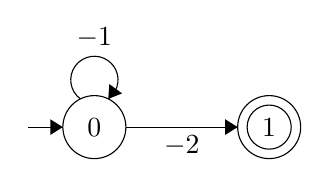
\begin{tikzpicture}[scale=0.2]
\tikzstyle{every node}+=[inner sep=0pt]
\draw [black] (4.4,-6.8) circle (2);
\draw (4.4,-6.8) node {$0$};
\draw [black] (15.5,-6.8) circle (2);
\draw (15.5,-6.8) node {$1$};
\draw [black] (15.5,-6.8) circle (1.4);
\draw [black] (0.2,-6.8) -- (2.4,-6.8);
\fill [black] (2.4,-6.8) -- (1.6,-6.3) -- (1.6,-7.3);
\draw [black] (3.518,-5.014) arc (234:-54:1.5);
\draw (4.4,-1.8) node [above] {$-1$};
\fill [black] (5.28,-5.01) -- (6.16,-4.66) -- (5.35,-4.07);
\draw [black] (6.4,-6.8) -- (13.5,-6.8);
\fill [black] (13.5,-6.8) -- (12.7,-6.3) -- (12.7,-7.3);
\draw (9.95,-7.3) node [below] {$-2$};
\end{tikzpicture}
\caption{The original environment.}
\end{subfigure}
\begin{subfigure}{0.3 \textwidth}
\centering
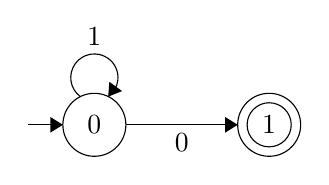
\begin{tikzpicture}[scale=0.2]
\tikzstyle{every node}+=[inner sep=0pt]
\draw [black] (4.4,-6.8) circle (2);
\draw (4.4,-6.8) node {$0$};
\draw [black] (15.5,-6.8) circle (2);
\draw (15.5,-6.8) node {$1$};
\draw [black] (15.5,-6.8) circle (1.4);
\draw [black] (0.2,-6.8) -- (2.4,-6.8);
\fill [black] (2.4,-6.8) -- (1.6,-6.3) -- (1.6,-7.3);
\draw [black] (3.518,-5.014) arc (234:-54:1.5);
\draw (4.4,-1.8) node [above] {$1$};
\fill [black] (5.28,-5.01) -- (6.16,-4.66) -- (5.35,-4.07);
\draw [black] (6.4,-6.8) -- (13.5,-6.8);
\fill [black] (13.5,-6.8) -- (12.7,-6.3) -- (12.7,-7.3);
\draw (9.95,-7.3) node [below] {$0$};
\end{tikzpicture}
\caption{The environment after adding \(c=2\) to the rewards.}
\end{subfigure}
\end{figure}

In this example, state \(0\) is the starting state and state \(1\) is the termination state.
Before making rewards non-negative, the optimal policy was to go directly to the termination state, to suffer the least amount of negative reward.
But after making rewards non-negative, the optimal policy in state \(0\) is to stay there, to get the maximum reward.

\section{}
Policy evaluation:
\begin{align}
V_0^{\pi_{t}}(s) &= 0\\
V_{k+1}^{\pi_{t}}(s) &= \sum_{s'} P(s'|s,\pi_{t}(s)) \left[ R(s,\pi_{t}(s),s') + \gamma V_{k}^{\pi_{t}}(s') \right]
\end{align}
Policy improvement:
\begin{align}
\pi_{t+1}(s) &= \argmax_{a} \sum_{s'} P(s'|s,a) \left[ R(s,a,s') + \gamma V^{\pi_{t}}(s') \right]
\end{align}
I'll denote \(V_{\infty}^{\pi}\) with \(V^{\pi}\) in this question.
\subsection{}
Suppose \(V^{\pi_t} = V^{\pi_{t+1}}\).
We can show that the Bellman optimality equation holds for them, therefore we have reached the optimal policy.\\
We know that by letting \(k \to \infty\):
\begin{align*}
V^{\pi_{t+1}}(s) &= \sum_{s'} P(s'|s,\pi_{t+1}(s)) \left[ R(s,\pi_{t+1}(s),s') + \gamma V^{\pi_{t+1}}(s') \right]
\end{align*}
So we have:
\begin{align*}
V^{\pi_{t+1}}(s) &= \sum_{s'} P(s'|s,a^*) \left[ R(s,a^*,s') + \gamma V^{\pi_{t+1}}(s') \right]\\
\text{Where } a^* &= \argmax_{a} \sum_{s'} P(s'|s,a) \left[ R(s,a,s') + \gamma V^{\pi_{t}}(s') \right]\\
\implies V^{\pi_{t+1}}(s) &= \max_a \sum_{s'} P(s'|s,a) \left[ R(s,a,s') + \gamma V^{\pi_{t}}(s') \right]\\
\xRightarrow{V^{\pi_{t+1}} = V^{\pi_{t}}} V^{\pi_{t+1}}(s) &= \max_a \sum_{s'} P(s'|s,a) \left[ R(s,a,s') + \gamma V^{\pi_{t+1}}(s') \right]
\end{align*}

Thus, Bellman equation holds for \(V^{\pi_{t+1}}\) (and as a result, for \(\pi_{t}\)). So we have achieved the optimal policy.

\subsection{}
There can be \(\abs{A}^{\abs{S}}\) policies.
And we know in each iteration the value of states increase or stay the same.
And also we proved that if the \(V\) function of two consecutive policies are equal, then we have reached the optimal policy.
So we can have at most \(\abs{A}^{\abs{S}}\) iterations before reaching the optimal policy and the policy iteration algorithm converges.

\subsection{}
As we saw, the convergence of the policy iteration algorithm doesn't depend on the environment being episodic or continuous (i.e., non-terminating) like the value iteration algorithm (or gamma being less than one as in the proof with contraction mapping).

Moreover, the policy iteration usually concludes in much fewer iterations than the value iteration algorithm, which makes it more efficient in practice.

\subsection{}
\begin{align*}
V_{0}^{\pi_{t+1}}(s) &= \sum_{s'} P(s'|s, a^*)\left[ R(s,a^*,s') + \gamma V_{\infty}^{\pi_{t}}(s') \right]\\
\text{Where } a^* &= \argmax_{a} \sum_{s'} P(s'|s,a) \left[ R(s,a,s') + \gamma V_{\infty}^{\pi_{t}}(s') \right]\\
\implies V_{0}^{\pi_{t+1}}(s) &= \max_a \sum_{s'} P(s'|s,a) \left[ R(s,a,s') + \gamma V_{\infty}^{\pi_{t}}(s') \right]\\
\end{align*}
Also we know that:
\begin{align*}
V_{\infty}^{\pi_t} &= \sum_{s'} P(s'|s,\pi_t(s)) \left[ R(s,\pi_t(s),s') + \gamma V_{\infty}^{\pi_{t}}(s') \right]
\end{align*}
So obviously \(V_0^{\pi_{t+1}}(s)\) is larger than \(V_{\infty}^{\pi_t}(s)\) for all \(s\), because of the maximization over all actions that it has.

Now we know that \(\forall s, k:\ V_{k+1}^{\pi_{t+1}}(s) \ge V_{k}^{\pi_{t}}(s)\). Therefore:
\begin{align*}
\forall s:\ V_\infty^{\pi_{t+1}}(s) \ge \cdots \ge V_{0}^{\pi_{t+1}}(s) \ge V_{\infty}^{\pi_t}(s)
\end{align*}

And we know that the initial value we use for \(V\), i.e.  \(V_0^{\pi_{t+1}}\), doesn't affect the final value in the policy evaluation, \(V_\infty^{\pi_{t+1}}\).
Because \(V_\infty^{\pi_{t+1}}\) is the solution of the Bellman equation: \(V^{\pi_{t+1}}_\infty = R^{\pi_{t+1}} + \gamma P^{\pi_{t+1}} V^{\pi_{t+1}}_\infty \implies V^{\pi_{t+1}}_\infty = (I - \gamma P^{\pi_{t+1}})^{-1} R^{\pi_{t+1}}\).
So by starting from \(V_0^{\pi_{t+1}} = 0\) too, the inequality \(V_\infty^{\pi_{t+1}}(s) \ge  V_{\infty}^{\pi_t}(s)\) holds.

We can prove that with the following argument too:
\begin{align*}
\pi_{t+1}(s) &= \argmax_a Q^{\pi_{t}}(s,a)\\
\implies Q^{\pi_{t}}(s, \pi_{t+1}(s)) &\ge Q^{\pi_{t}}(s, \pi_{t}(s)) = V^{\pi_{t}}(s)    
\end{align*}
\begin{align*}
\implies V^{\pi_{t}}(s) &\le Q^{\pi_{t}}(s, \pi_{t+1}(s))\\
&= \E[\pi_{t+1}]{r_{1} + \gamma V^{\pi_{t}}(s_{1})|s_{0}=s}\\
&\le \E[\pi_{t+1}]{r_{1} + \gamma Q^{\pi_{t}}(s_{1}, \pi_{t+1}(s_{1}))|s_{0}=s}\\
&= \E[\pi_{t+1}]{r_{1} + \gamma \E[\pi_{t+1}]{r_{2} + \gamma V^{\pi_{t}}(s_{2})|s_{1}}|s_{0}=s}\\
&= \E[\pi_{t+1}]{r_{1} + \gamma r_{2} + \gamma^2 V^{\pi_{t}}(s_{2})|s_{0}=s}\\
&\le \E[\pi_{t+1}]{r_{1} + \gamma r_{2} + \gamma^2 Q^{\pi_{t}}(s_{2}, \pi_{t+1}(s_{2}))|s_{0}=s}\\
% & ... 
& \ \vdots\\ 
&\le \E[\pi_{t+1}]{r_{1} + \gamma r_{2} + \gamma^2 r_{3} + \cdots|s_{0}=s}\\
&= V^{\pi_{t+1}}(s)
\end{align*}

\section{}
\subsection{}
When we have two actions, the Gini index is \(p_1(1-p_1) + p_2(1-p_2) = 2p_1(1-p_1)\).
And it is maximized when \(p_1 = p_2 = 0.5\).
In general, the \(p(1-p)\) term in the sum, makes sure that none of the probabilities are too low or too high, or the \(p(1-p)\) term will be too small and the Gini index will be small.

\subsection{}
Aside from maximizing the mentioned term, we have to make sure that the sum of the probabilities is one:
\begin{align*}
\mathcal{L}(\pi, \lambda) &= \E[\pi]{r(a)} + \beta \Gini (\pi) + \lambda (1 - \sum_{a} \pi(a))\\
&= \sum_{a \in A} \pi(a) r(a) + \beta \sum_{a \in A} \pi(a) (1 - \pi(a)) + \lambda (1 - \sum_{a} \pi(a))\\
&= \lambda + \sum_{a \in A} \pi(a) r(a) + \beta \pi(a) - \beta \pi(a)^2 - \lambda \pi(a)
\end{align*}

\subsection{}
\begin{align*}
\mathcal{L}(\pi, \lambda) &= \lambda + \sum_{a \in A} \pi(a) r(a) + \beta \pi(a) - \beta \pi(a)^2 - \lambda \pi(a)\\
\frac{\partial \mathcal{L}}{\partial \pi(a)} &= r(a) + \beta - 2\beta \pi(a) - \lambda = 0\\
\implies \pi(a) &= \frac{r(a) + \beta - \lambda}{2\beta}
\end{align*}
\begin{align*}
\frac{\partial \mathcal{L}}{\partial \lambda} &= 1 - \sum_{a \in A} \pi(a) = 0\\
\implies& \sum_{a \in G} \frac{r(a) + \beta - \lambda}{2\beta} = 1\\
\implies& \sum_{a \in G} r(a) + \beta - \lambda = 2\beta\\
\implies&  \abs{G} (\beta - \lambda) = 2\beta - \sum_{a \in G} r(a)\\
\implies& \lambda = \beta - \frac{2\beta - \sum_{a \in G} r(a)}{\abs{G}}
\end{align*}
\begin{align*}
\implies \pi(a) &= \frac{\abs{G} r(a) + 2\beta - \sum_{a \in G} r(a)}{2\beta \abs{G}}
\end{align*}

\subsection{}
The objective of quadratic programming is to find an n-dimensional vector \(x\) such that:
\begin{align*}
\text{minimize }& \frac{1}{2} x^T Q x + c^T x\\
\text{subject to }& Ax \le b    
\end{align*}
We can define a QP problem to find the optimal policy and \(G\) along with it.
\begin{align*}
R&: \text{vector of rewards for each action}\\
x&: \text{vector of probabilities for each action}\\
\mathbb{1}_n \text{ and }\mathbb{0}_n&: \text{vector of ones and zeros of size } n
\end{align*}
We can rewrite our objective function as:
\begin{align*}
\text{maximize }& R^T x + \beta \mathbb{1}_n^T x - \beta x^T I x\\
\text{subject to }& - I x \preceq 0\\
& \ \ \  \mathbb{1}_n^T x \preceq 1\\
& - \mathbb{1}_n^T x \preceq 1\\
\end{align*}
Where two last conditions are to make sure that the sum of the probabilities is one.
We can define \(Q\), \(c\), \(A\) and \(b\) for our QP problem as:

\begin{align*}
Q &= 2\beta I_n\\
c &= -R - \beta \mathbb{1}\\
A &= \begin{bmatrix}
    - I_n\\
    \mathbb{1}_n^T\\
    - \mathbb{1}_n^T
\end{bmatrix}\\
b &= \begin{bmatrix}
    \mathbb{0}_n\\
    1\\
    1
\end{bmatrix}
\end{align*}
Solving this QP problem will give us the optimal policy.\\
We can also find \(G\) simply as \(\left\{a: \pi(a) > 0\right\}\).

\section{}
\subsection{}
\begin{align*}
E_t(s) &= \gamma \lambda E_{t-1}(s) + I_{ss_t}\\
&= (\gamma \lambda)^2 E_{t-2}(s) + (\gamma \lambda) I_{ss_t} + I_{ss_t}\\
&= \cdots\\
&= (\gamma \lambda)^t I_{ss_0} + \cdots + (\gamma \lambda) I_{ss_t} + I_{ss_t}\\
&= \sum_{k=0}^{t} (\gamma \lambda)^{t-k} I_{ss_k}
\end{align*}

\subsection{}
\begin{align*}
\Delta V_t^{TD}(s) &= \alpha \delta_t E_t(s)\\
\implies \sum_{t=0}^{T-1} \Delta V_t^{TD}(s) &= \sum_{t=0}^{T-1} \alpha \delta_t E_t(s)\\
&= \sum_{t=0}^{T-1} \alpha \delta_t \sum_{k=0}^{t} (\gamma \lambda)^{t-k} I_{ss_k}\\
\xrightarrow{\text{swapping the sums}} &= \sum_{k=0}^{T-1} \sum_{t=k}^{T-1} \alpha \delta_t (\gamma \lambda)^{t-k} I_{ss_k}\\
\xrightarrow{\text{swapping }t, k} &= \sum_{t=0}^{T-1} \sum_{k=t}^{T-1} \alpha \delta_k (\gamma \lambda)^{k-t} I_{ss_t}\\
&= \sum_{t=0}^{T-1} \alpha I_{ss_t} \sum_{k=t}^{T-1} (\gamma \lambda)^{k-t} \delta_k
\end{align*}

\subsection{}
\begin{align*}
\frac{1}{\alpha} \Delta V_t^\lambda (s_t) &= G_t^\lambda - V_t(s_t)\\
&= -V_t(s_t) + (1-\lambda) \sum_{n=1} \lambda^{n-1} G_t^n\\
&= -V_t(s_t) + (1-\lambda) \left[ \lambda^0 \left[ r_{t+1} + \gamma V_t(s_{t+1}) \right] + \lambda^1 \left[ r_{t+1} + \gamma r_{t+2} + \gamma^2 V_t(s_{t+2}) \right] + \cdots \right]\\
&= -V_t(s_t) + (1-\lambda) \left[ \left(\lambda^0 + \lambda^1 + \cdots \right) r_{t+1} + \left(\lambda^1 + \lambda^2 + \cdots \right) \gamma r_{t+2} + \cdots \right]\\
& \hspace*{2in} + \sum_{k=t}^{\infty} \gamma (1-\lambda) (\gamma \lambda)^{k-t} V_t(s_{k+1})\\
&= -V_t(s_t) + \left[\lambda^0 r_{t+1} + (\lambda \gamma)^1 r_{t+2} + \cdots\right]
+ \sum_{k=t}^{\infty} \left(\gamma \lambda\right)^{k-t} \left( \gamma V_t(s_{k+1}) - \gamma \lambda V_t(s_{k+1}) \right)\\
\xrightarrow{\text{including } -V_t(s_t) \text{in sum}}&= \sum_{k=t}^{\infty} (\gamma \lambda)^{k-t} r_{k+1} + \sum_{k=t}^{\infty} (\gamma \lambda)^{k-t} \gamma V_t(s_{k+1}) - V_t(s_k)\\
&= \sum_{k=t}^{\infty} (\gamma \lambda)^{k-t} \left[ r_{k+1} + \gamma V_t(s_{k+1})  - V_t(s_k)\right]
\end{align*}

\subsection{}
\begin{align*}
\frac{1}{\alpha} \Delta V_t^\lambda (s_t) &= \sum_{k=t}^{\infty} (\gamma \lambda)^{k-t} \left[ r_{k+1} + \gamma V_t(s_{k+1}) - V_t(s_k)\right]\\
&\approx \sum_{k=t}^{\infty} (\gamma \lambda)^{k-t} \delta_k\\
&\approx \sum_{k=t}^{T - 1} (\gamma \lambda)^{k-t} \delta_k
\end{align*}
These approximations will be equality in offline update case.
Because in offline case, \(V_t\) is equal for all \(t\), and also all steps after the terminal states have zero reward and zero values, and we can omit them from the summation.

\end{document}